Modelling phase is critical. Starting from a new problem and observing it by different \textbf{perspectives} we can design several models. Generally, every
model exhibits a different representation of the original problem, in particular any of them have:
\begin{enumerate}
    \item Different decision variables.
    \item Different domains.
    \item Different constraints.
    \item Different size of the search space.
\end{enumerate}
Which model is the best one?
\begin{example}[title = Symmetries of n-queens problem]
    e.g. Solution of n-queens problem. \vspace{3.5pt}
    \begin{center}
        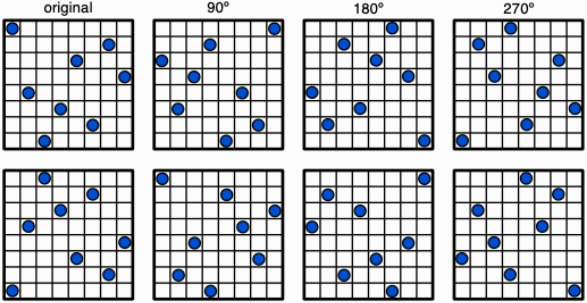
\includegraphics[width = 0.5\textwidth]{img/img8.png}
    \end{center} \vspace{3.5pt}
    Just rotating and flipping the board we end up with \textit{seven} additional symmetric solutions of the top-left original one. Additionally, 
    we cannot impose an ordering constraint as we did before for the ruler problem. We need a new \textbf{viewpoint} to avoid these \textit{seven} symmetric 
    feasible solutions. \vspace{7pt}

    \textbf{Decision variables and domains}. \\ 
    We represent the $n \times n$ board as a boolean board and every decision variable is a boolean variable like $B_{ij} \in \{0,1\}$. \vspace{7pt}

    \textbf{Attacking constraints}.
    \begin{itemize}
        \renewcommand{\labelitemi}{-}
        \item $\sum B_{ij} = 1$ on all rows and columns.
        \item $\sum B_{ij} \leq 1$ on all the diagonals.
    \end{itemize} \vspace{7pt}
    
    Now we are able to convert geometric symmetry to boolean symmetry. \vspace{7pt}

    \textbf{Symmetry breaking constraints}. \\
    We determine the following list of steps to avoid symmetric solutions. 
    \begin{enumerate}
        \item Flat the 2-D matrix to a single sequence of variables. Simply, we take each row of the board and we append it at the end of the sequence.
        \item Every symmetric configuration corresponds to a \textbf{variable permutation} of the original solution, which is easy to define.
        \item We then impose an order between a solution and all the solutions obtained by the \textit{seven} permutations:
        $$ \textit{lex} \leq (B, \pi(B)) \text{ for all } \pi $$
        where: 
        \begin{itemize}
            \renewcommand{\labelitemi}{-}
            \item $B \rightarrow$ flatten version of the 2-D matrix
            \item $\pi(B) \rightarrow$ symmetries of the original solution
        \end{itemize}
    \end{enumerate}
\end{example} 